\documentclass[11pt]{article}

\usepackage[margin=1in]{geometry}
\usepackage{amsmath}
\usepackage{amssymb}
\usepackage{booktabs}
\usepackage{enumitem}
\usepackage{graphicx}
\usepackage{xcolor}
\usepackage{hyperref}
\usepackage{url}

\setlist{nosep,leftmargin=*}
\setlength{\textfloatsep}{8pt plus 2pt minus 2pt}
\setlength{\floatsep}{6pt plus 2pt minus 2pt}
\setlength{\intextsep}{6pt plus 2pt minus 2pt}

\hypersetup{
  colorlinks=true,
  linkcolor=blue,
  citecolor=blue,
  urlcolor=blue
}

\newcommand{\Dpos}{\mathcal{D}^{+}}
\newcommand{\Dneg}{\mathcal{D}^{-}}
\newcommand{\Dunl}{\mathcal{D}^{u}}
\newcommand{\clip}{\operatorname{clip}}
\newcommand{\method}{TRIAGE-BC}

\title{When Do Bad Demonstrations Help Offline Imitation? A Precision-Coverage Study}
\author{Anonymous Authors}
\date{}

\begin{document}
\maketitle

\begin{abstract}
Offline imitation datasets often mix scarce trusted successes, scarce known failures, and larger unlabeled logs. We study when failure demonstrations help as a score-to-support conversion problem: failures can calibrate a desirability score, but policy quality depends on converting scores into behavior-cloning support. \method{} learns a tri-signal state-action score, estimates hidden positive mass, and routes unlabeled data into hard support, soft weighting, or abstention. Controlled PointNav and targeted generated Robomimic Can diagnostics show explicit failures help when positives are incomplete, trusted positives under-cover the state distribution, or bad demos are action-conflicting near-neighbors. A frozen v0.2 portfolio reaches 209/300 fresh Can+Lift successes versus 187/300 for best per-split non-oracle baselines by choosing hard union on Can and weighted coverage on Lift. The evidence supports a focused conclusion: bad labels can calibrate useful support, but hidden-label-free conversion from scores to policy-training data remains the bottleneck, and strong positive-only and weighted baselines must remain first-class controls.
\end{abstract}

\section{Introduction}

Offline imitation learning is often presented as a problem of cloning desirable demonstrations. In many practical settings, however, the available data is not a clean demonstration set. A user may have a handful of trusted successes, a handful of known failures, and a much larger log whose behavior is unlabeled and mixed. Some of that log may contain useful recoveries, alternate strategies, or broader state coverage; some may contain shortcuts, failed attempts, or actions that conflict with the desired behavior.

The simplest responses are unsatisfactory. Cloning all available trajectories can reproduce harmful behavior. Cloning only the scarce successes can be high precision but low coverage. Softly weighting unlabeled trajectories by a learned desirability score can preserve coverage, but it can also keep too much action-conflicting bad behavior in the policy-training distribution. Hard filtering can remove bad trajectories, but it can also discard coverage that a sequence policy needs to solve the task.

This paper studies the conversion step between score learning and policy learning. Given scarce successes, scarce failures, and a mixed unlabeled log, the central question is not merely whether a classifier can separate good from bad transitions. The central question is how its scores should become a policy-training distribution.

We propose \method{}, a score-calibrated behavior cloning framework. \method{} trains a state-action desirability classifier from labeled successes and failures, aggregates classifier probabilities into trajectory scores, estimates positive mass in the unlabeled log from labeled score anchors, and then routes the unlabeled data through a hidden-label-free support converter. The frozen v0.1 method uses hard adaptive mass-capped support, positive-minimum threshold support, and abstention for ambiguous high-mass score shapes. The frozen v0.2 portfolio adds an explicit hard-risk-union branch, a soft weighted branch, and stress abstention, chosen by score-derived mass and coverage features.

Our results support a narrower story than a full inverse-reward or inverse-Q claim. In controlled PointNav, where positive labels are only route prefixes and the unlabeled log contains hidden full routes mixed with trap shortcuts, adaptive score-gap support recovers useful hidden support and reaches perfect success under heavy contamination. In Robomimic \cite{mandlekar2021robomimic}, v0.1 reveals the precision/coverage failure modes: positive-only retrieval is strongest on the original Can 40p/80b matrix, while weighted BC is strongest on the original Lift MG matrix. The frozen v0.2 router then passes a fresh Can+Lift gate, reaching 209/300 selected-branch successes versus 187/300 for the best per-split non-oracle baselines. Can carries the cleaner improvement; Lift is a modest branch-selection result because v0.2 selects weighted BC and loses one split.

The contributions are:
\begin{enumerate}[leftmargin=*]
  \item We formalize offline imitation from scarce successes, scarce failures, and a contaminated unlabeled log as a score-to-support conversion problem.
  \item We introduce \method{} v0.1, a hidden-label-free tri-signal support calibration baseline, and a frozen v0.2 portfolio router over hard union, soft weighting, and abstention.
  \item We provide controlled PointNav and generated Robomimic Can diagnostics showing when explicit failures help: incomplete positives, action-conflicting near-neighbor failures, and scarce-positive coverage shift.
  \item We report frozen Robomimic endpoint evidence and caveats: Can 40p/80b favors hard selected support, Lift MG favors weighted coverage, positive-only retrieval remains strong, and all claims are checked against artifact maps.
\end{enumerate}

\section{Related Work}

\paragraph{Imitation learning.}
Behavior cloning is the standard supervised-learning baseline for imitation learning, but sequential prediction suffers when the learned policy visits states not represented in the demonstrations. Interactive methods such as DAgger address this by querying an expert on learner-induced states \cite{ross2011dagger}, while broader surveys emphasize the role of dataset coverage and distribution shift in imitation learning \cite{osa2018algorithmic}. \method{} remains offline: it assumes no expert queries, no online data collection, and no online reward optimization.

\paragraph{Inverse reinforcement learning and adversarial imitation.}
Classical inverse reinforcement learning infers a reward that explains expert behavior \cite{ng2000irl}, with apprenticeship learning and maximum-entropy variants providing influential formulations \cite{abbeel2004apprenticeship,ziebart2008maxent}. Adversarial imitation methods such as GAIL instead match expert occupancy through an adversarial objective \cite{ho2016gail}. These approaches usually use the inferred reward, discriminator, or occupancy objective to extract a policy through additional optimization. The current paper should not be read as validating a full inverse-Q robotics method. The robotics evidence uses a score-calibrated data converter followed by official Robomimic BC-RNN-GMM policy learning.

\paragraph{Offline RL and advantage-weighted imitation.}
Offline RL benchmarks and algorithms study policy improvement from static datasets with no environment interaction \cite{fu2020d4rl}. Conservative Q-learning regularizes value estimates to avoid unsupported action overestimation \cite{kumar2020cql}. IQL extracts policies through advantage-weighted behavior cloning after value learning \cite{kostrikov2022iql}; AWR and AWAC also use weighted maximum-likelihood policy updates over off-policy data \cite{peng2019awr,nair2020awac}. \method{} differs in its supervision: it uses scarce positive and negative demonstration labels to calibrate support from a mixed log, rather than using task rewards to estimate advantages.

\paragraph{Positive-unlabeled and data-selection views.}
The problem is related to positive-unlabeled learning, where classifiers are learned from trusted positives and a mixed unlabeled pool \cite{elkan2008positive}. Our setting adds explicit negative demonstrations and a downstream policy-learning objective. Recent work on data quality in imitation learning also shows that which demonstrations are included can matter as much as the cloning objective itself \cite{belkhale2023dataquality}. The key empirical lesson here is more specific: classification quality is insufficient by itself because a selected support set must also contain the coverage needed by the policy learner.

\paragraph{Robotics demonstration quality and sequence backbones.}
Robomimic studies offline robot manipulation from human demonstrations and emphasizes controlled data, architectures, and evaluation protocols for sequence imitation \cite{mandlekar2021robomimic}. Our robotics experiments inherit this lesson by using the same official BC-RNN-GMM backbone across methods and by fixing endpoint checkpoints. The contribution is therefore not a new robot policy architecture. It is the calibrated conversion of scarce positive and failure labels into the support used by a standard sequence cloning policy, with positive-only retrieval and all-positive oracles included as necessary controls.

\section{Problem Setting}

The learner receives three offline trajectory sets:
\begin{align}
  \Dpos &= \{\tau_i^+\}_{i=1}^{n_+}, &
  \Dneg &= \{\tau_i^-\}_{i=1}^{n_-}, &
  \Dunl &= \{\tau_i^u\}_{i=1}^{n_u}.
\end{align}

\noindent $\Dpos$ contains scarce trusted successful or desirable demonstrations. $\Dneg$ contains scarce known failed or undesirable demonstrations. $\Dunl$ is a larger unlabeled mixed-quality log. No online training interaction is allowed. The method may use membership in $\Dpos$ and $\Dneg$, but it may not use hidden labels inside $\Dunl$ for score training, threshold selection, branch selection, checkpoint selection, or policy training. Hidden labels and task rewards are reserved for audits, oracle diagnostics, and evaluation.

The objective is to train a policy that behaves like the desirable behavior represented by $\Dpos$, while using $\Dunl$ when it contains useful state-action coverage and avoiding imitation of undesirable behavior represented by $\Dneg$. The main method output is a policy-training distribution, not a reward function used for online reinforcement learning.

\section{Method}

Figure~\ref{fig:pipeline} summarizes the \method{} pipeline. The frozen v0.1 method contract is stored in \path{../METHOD_FREEZE.md}.

\begin{figure}[t]
  \centering
  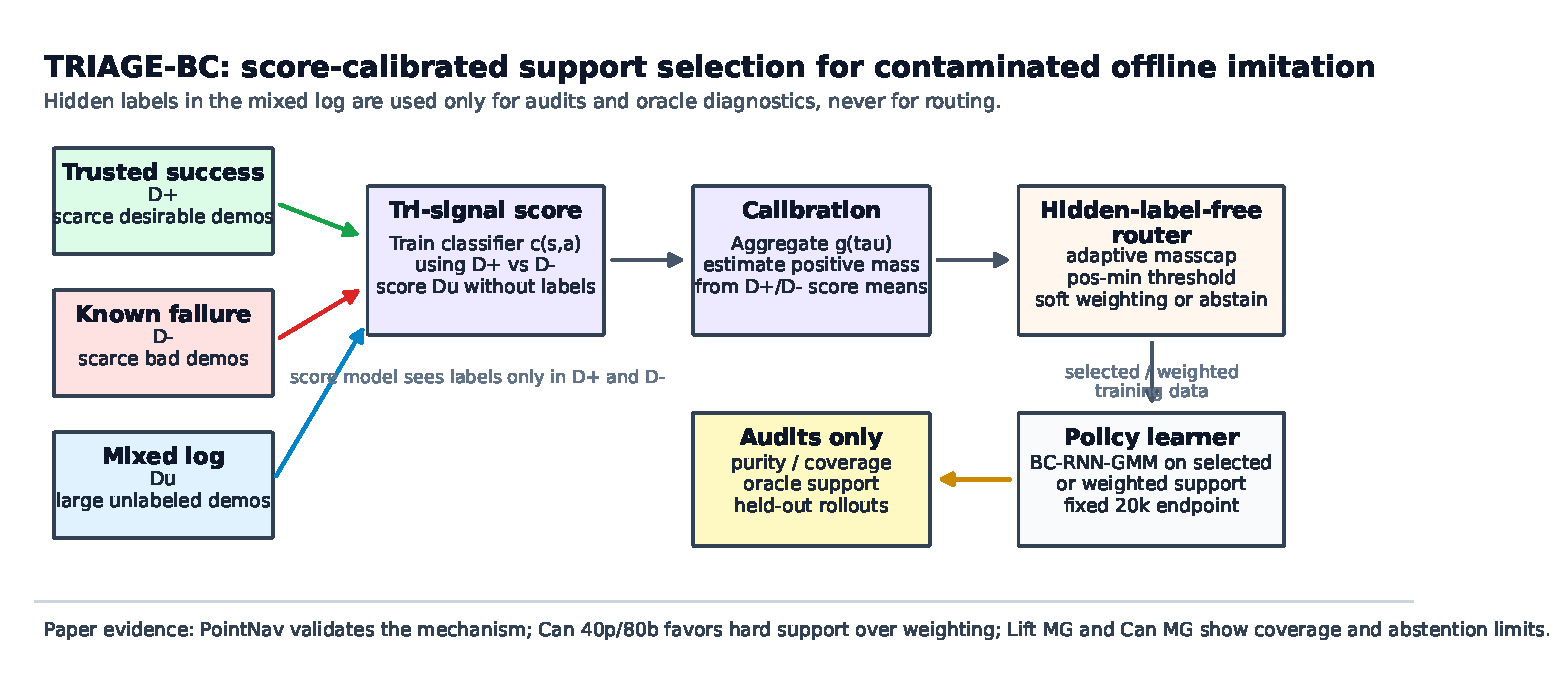
\includegraphics[width=\linewidth]{../results/final_paper/figures/triage_bc_method_diagram.pdf}
  \caption{\method{} learns a tri-signal score from scarce positives and failures, aggregates scores over unlabeled trajectories, converts scores into policy-training support, and audits hidden labels only after evaluation.}
  \label{fig:pipeline}
\end{figure}

\subsection{Tri-Signal Score Learning}

\method{} trains a binary state-action classifier
\begin{equation}
  c_\theta(s,a) \in [0, 1],
\end{equation}
where transitions from $\Dpos$ are labeled 1 and transitions from $\Dneg$ are labeled 0. Unlabeled transitions from $\Dunl$ are not used to train the score model. The score loss is
\begin{equation}
  \mathcal{L}_{\mathrm{score}}
  =
  -\mathbb{E}_{(s,a)\sim\Dpos}\log c_\theta(s,a)
  -\mathbb{E}_{(s,a)\sim\Dneg}\log(1-c_\theta(s,a)).
\end{equation}

For Robomimic, the frozen implementation uses observation-action features, 800 classifier steps, batch size 512, hidden dimension 128, depth 2, learning rate $10^{-4}$, and sigmoid output probabilities.

\subsection{Trajectory Score Calibration}

For each trajectory $\tau$, \method{} computes the mean trajectory score
\begin{equation}
  g(\tau) = \frac{1}{|\tau|}\sum_{(s_t,a_t)\in\tau} c_\theta(s_t,a_t).
\end{equation}
Diagnostics also record score minima, percentiles, and histograms, but the frozen method uses the mean score for support conversion.

Let
\begin{equation}
  \mu_+ = \frac{1}{|\Dpos|}\sum_{\tau\in\Dpos} g(\tau),
  \qquad
  \mu_- = \frac{1}{|\Dneg|}\sum_{\tau\in\Dneg} g(\tau).
\end{equation}
The hidden-label-free estimated positive mass in $\Dunl$ is
\begin{equation}
  p_u(\tau)
  =
  \clip\left(
    \frac{g(\tau)-\mu_-}{\mu_+-\mu_-+\epsilon},
    0, 1
  \right),
  \qquad
  \hat{m} = \sum_{\tau\in\Dunl} p_u(\tau).
\end{equation}

\subsection{Support Conversion}

\method{} v0.1 uses a small family of support converters:
\begin{itemize}[leftmargin=*]
  \item \textbf{Adaptive mass-capped hard support}: sort $\Dunl$ by $g(\tau)$, compute score-gap support subject to a minimum count, estimate $\hat{m}$, and cap support when the gap-selected set is too broad relative to $\hat{m}$.
  \item \textbf{Positive-minimum support}: select unlabeled trajectories whose score exceeds the minimum labeled-positive trajectory score.
  \item \textbf{Weighted sampler}: train on $\Dpos \cup \Dunl$ with labeled positives weighted as 1 and unlabeled demos weighted by their score. In v0.1 this is a required baseline and diagnostic branch rather than the main router output.
  \item \textbf{Positive-only NN control}: select unlabeled demos nearest to labeled positives without using $\Dneg$. This is a required no-bad-label baseline, not \method{}.
\end{itemize}

\subsection{Frozen Router}

The paper-facing router chooses between hard support and abstention using only score-shape features:
\begin{enumerate}[leftmargin=*]
  \item Compute $\hat{m}$, the number of unlabeled trajectories above the minimum labeled-positive score, and the tenth percentile of labeled-positive trajectory scores.
  \item If $\hat{m}\ge 800$ and at least 400 unlabeled trajectories exceed the positive-minimum threshold, abstain and report the split as a stress diagnostic.
  \item Else if the labeled-positive tenth percentile is at least 0.85 and at least 80 unlabeled trajectories exceed the positive-minimum threshold, use positive-minimum hard support.
  \item Else use adaptive mass-capped hard support.
\end{enumerate}
The router does not choose weighted BC as the main method branch in v0.1. Weighted BC remains a same-backbone baseline and a diagnostic branch for abstained Can MG-style splits.

\subsection{Frozen v0.2 Portfolio Router}

After the v0.1 diagnostics, we froze a small v0.2 portfolio router before fresh Can 40p/80b and Lift MG split seeds 101, 202, and 303. It reuses the score model and routes by two unlabeled score-shape features: estimated positive mass $\hat{m}$ and the count above the labeled-positive minimum score. Very large mass and count trigger stress abstention; moderate mass/count selects classifier-probability weighted BC with weights clipped below by 0.05; otherwise the router selects hard positive-NN/risk-union support. The hard branch unions positive-only nearest-neighbor support with a rank-fusion support set combining positive-neighbor rank and bad-aware action-risk rank. Branch selection uses no hidden unlabeled labels, and the result is a portfolio converter rather than a claim that one fixed threshold is universally best.

\subsection{Algorithmic Summary}

The frozen \method{} v0.1 procedure is:
\begin{enumerate}[leftmargin=*]
  \item Split the offline data into scarce labeled positives $\Dpos$, scarce labeled negatives $\Dneg$, unlabeled mixed trajectories $\Dunl$, and held-out positive evaluation starts.
  \item Train $c_\theta(s,a)$ only on transitions from $\Dpos$ and $\Dneg$.
  \item Score every trajectory with $g(\tau)$, compute labeled score anchors $\mu_+$ and $\mu_-$, and estimate unlabeled positive mass $\hat{m}$.
  \item Compute hidden-label-free score-shape features: $\hat{m}$, the count of unlabeled trajectories above the minimum labeled-positive score, and the tenth percentile of labeled-positive trajectory scores.
  \item Route the split. Large high-mass plateaus are abstained from; high positive-minimum score shapes use positive-minimum hard support; all other non-abstained splits use adaptive mass-capped hard support.
  \item Train the policy with the frozen BC backbone on the selected support. For Robomimic this is official BC-RNN-GMM at a fixed 20k optimizer-step endpoint.
  \item Report endpoint rollouts without best-checkpoint selection. Hidden labels are used only afterward for audit metrics such as selected-support purity, hidden-positive recall, and hidden-bad admission.
\end{enumerate}

\subsection{Policy Learning}

For Robomimic, policies are trained with official BC-RNN-GMM: sequence length 10, two-layer LSTM with hidden dimension 400, actor MLP dimensions 1024/1024, five GMM modes, 200 epochs with 100 steps per epoch, and fixed endpoint reporting at epoch 200. This is 20k optimizer steps. No rollout is used during training, and no best-checkpoint selection is used for main claims.

For controlled PointNav, the policy learner is a lightweight behavior cloning policy trained on the selected or weighted support. PointNav is used to isolate the support-recovery mechanism, not to claim robotics-scale policy learning.

\section{Experiments}

\subsection{Controlled Continuous PointNav}

The controlled PointNav task is designed so that positive labels alone are incomplete. Labeled positives are safe-route prefixes, while unlabeled trajectories contain hidden safe full routes and hidden shortcut failures. The method must recover useful hidden trajectories from the mixed log to solve the full route.

The strongest controlled setting uses only two positive prefixes and two bad shortcut trajectories. Score-gap support reaches 1.000 success at 50\%, 75\%, 90\%, and 95\% bad unlabeled data. All-demo cloning, positive-plus-unlabeled cloning, and local weighted BC degrade as contamination rises. Figure~\ref{fig:pointnav} shows the staged mechanism result.

\begin{figure}[t]
  \centering
  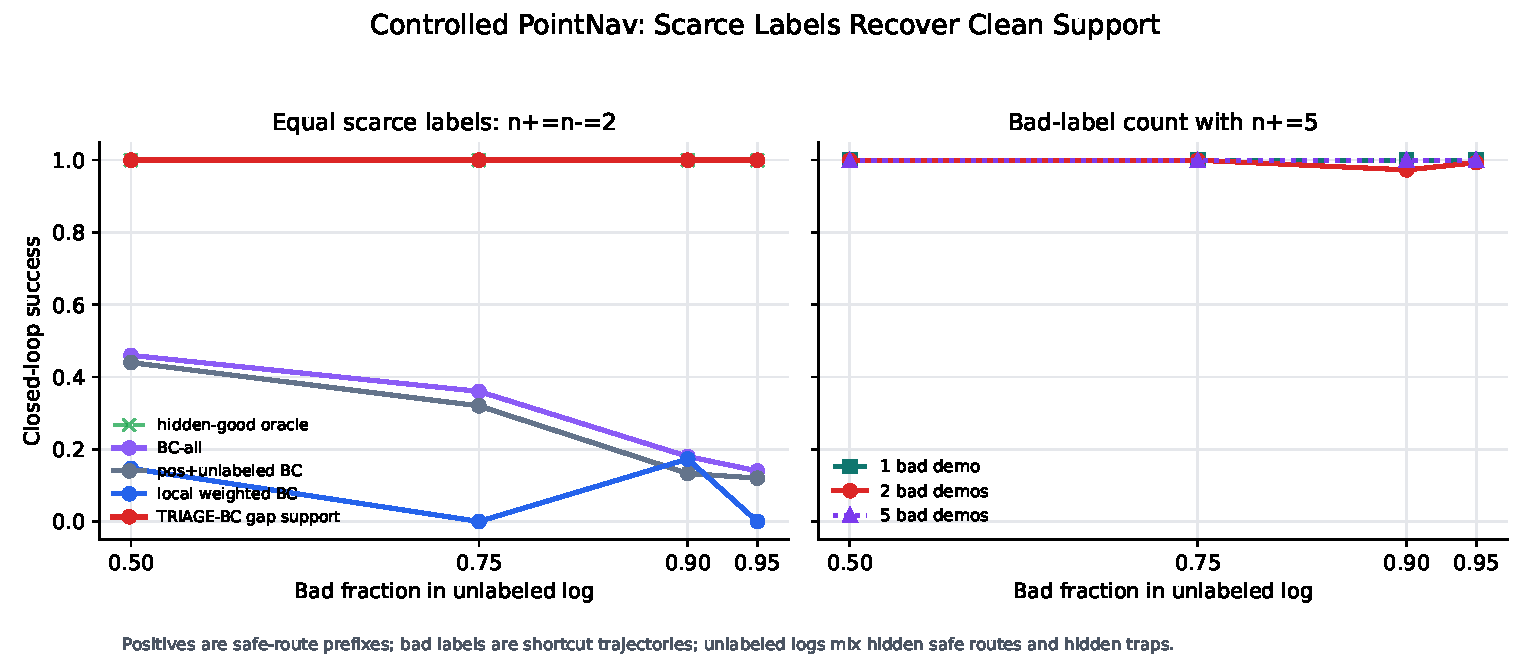
\includegraphics[width=\linewidth]{../results/final_paper/figures/pointnav_controlled_mechanism.pdf}
  \caption{Controlled PointNav mechanism result. Scarce bad labels calibrate support recovery when scarce positives only cover route prefixes.}
  \label{fig:pointnav}
\end{figure}

\subsection{Robomimic Frozen Endpoint Matrix}

Robomimic experiments use low-dimensional official BC-RNN-GMM policies trained under the frozen method contract. Final endpoint evaluation uses 50 held-out validation-positive rollouts per split and fixed epoch-200 checkpoints. The v0.1 primary frozen rows are Can 40p/80b and Lift MG, each over split seeds 11, 22, and 33. The v0.2 fresh gate uses split seeds 101, 202, and 303 for Can 40p/80b and Lift MG. Can 20p/80b, Can 80p/80b, and Can MG are diagnostic rows rather than complete main claims.

The key baselines are all-demo BC, classifier-probability weighted BC, positive-only NN, all-positive oracle, and classifier top-k support sweeps. Weighted BC is treated as a strong baseline, not as a strawman. Positive-only NN is also a strong baseline and is often the best non-oracle method on Can.

\section{Results}

\subsection{Controlled PointNav Mechanism Result}

Controlled PointNav is the clearest mechanism test because the labeled positives
are intentionally incomplete. With only two positive route-prefix demonstrations
and two bad shortcut demonstrations, score-gap support reaches 1.000 success at
50\%, 75\%, 90\%, and 95\% bad unlabeled data. All-demo cloning,
positive-plus-unlabeled cloning, and local weighted BC degrade as contamination
rises. This result supports the mechanism claim: scarce explicit bad labels can
calibrate support recovery when positives do not cover complete successful
behavior.

This result should not be read as a robotics-scale dominance claim. It isolates
why tri-signal calibration can be useful: the classifier score is valuable only
after it is converted into a policy-training support set that recovers hidden
safe full trajectories while rejecting shortcut failures.

\subsection{Robomimic Endpoint Results}

Figure~\ref{fig:matrix} and Table~\ref{tab:main-results} summarize the current primary frozen endpoint matrix.

\begin{figure}[t]
  \centering
  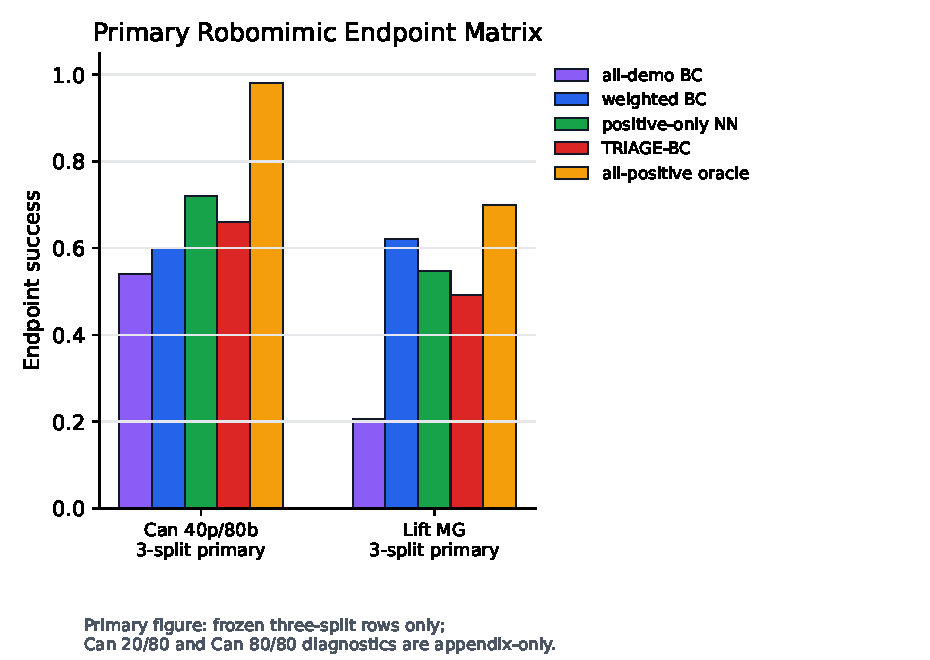
\includegraphics[width=\linewidth]{../results/final_paper/figures/robotics_primary_endpoint_matrix.pdf}
  \caption{Primary Robomimic endpoint matrix. Can 40p/80b and Lift MG are the completed frozen three-split aggregates. Can 20p/80b and Can 80p/80b are kept as diagnostic appendix evidence rather than main-figure rows.}
  \label{fig:matrix}
\end{figure}

\begin{table}[t]
  \centering
  \caption{Main frozen endpoint aggregates. Counts are successes over endpoint rollouts at epoch 200.}
  \label{tab:main-results}
  \begin{tabular}{lcc}
    \toprule
    Method & Can 40p/80b & Lift MG \\
    \midrule
    All-positive oracle & 147/150 & 105/150 \\
    Positive-only NN & 108/150 & 82/150 \\
    \method{} & 99/150 & 74/150 \\
    Weighted BC & 90/150 & 93/150 \\
    All-demo BC & 81/150 & 31/150 \\
    \bottomrule
  \end{tabular}
\end{table}

On Can 40p/80b, \method{} improves over weighted BC and all-demo cloning at the fixed 20k endpoint. This supports the claim that hard support can beat soft weighted sampling under action-conflicting contamination. However, positive-only NN top40 is the best non-oracle row, so Can 40p/80b does not support a claim that bad labels are necessary or that \method{} beats strong no-bad-label retrieval.

On Lift MG, all-demo cloning is weak, confirming that contaminated logs can hurt. But weighted BC is strongest among non-oracle rows. \method{} improves support purity, yet fixed endpoint policy performance trails broader coverage-sensitive baselines. This is a useful counterexample: high-purity hard support is not automatically the best policy-training distribution.

The primary endpoint uncertainty summary reinforces this cautious interpretation. On Can 40p/80b, \method{} beats weighted BC on all three splits, but the paired-bootstrap delta is modest, $+0.060$ with interval $[-0.113,0.240]$, and positive-only NN is higher pooled. On Lift MG, weighted BC is higher pooled than \method{}, with paired-bootstrap delta $+0.122$ and interval $[-0.100,0.317]$. The evidence is therefore directional and coverage-sensitive rather than a formal significance claim; the only primary paired-bootstrap interval strictly above zero is \method{} over all-demo BC on Lift MG, $[0.211,0.400]$.

\subsection{Fresh v0.2 Portfolio Gate}

Table~\ref{tab:v02-gate} summarizes the frozen v0.2 fresh-split gate. The router chooses hard positive-NN/risk-union support on Can 40p/80b and wins all three fresh splits; it chooses soft weighted BC on Lift MG and wins two of three, losing split 303 to positive-only NN. The combined gate is 209/300 selected-branch successes versus 187/300 for the best completed non-oracle baseline per split, so the interpretation is branch selection rather than universal hard-support dominance.

\begin{table}[t]
  \centering
  \caption{Frozen v0.2 fresh endpoint gate. Counts are successes over 50 endpoint rollouts per split at epoch 200.}
  \label{tab:v02-gate}
  \begin{tabular}{lccc}
    \toprule
    Setting & v0.2 selected branch & Best baseline per split & Split margins \\
    \midrule
    Can 40p/80b & 129/150 & 113/150 & +8/50, +5/50, +3/50 \\
    Lift MG & 80/150 & 74/150 & +3/50, +5/50, -2/50 \\
    Combined & 209/300 & 187/300 & 5 wins / 1 loss \\
    \bottomrule
  \end{tabular}
\end{table}

Paired initial-state bootstraps remain descriptive and cross zero for Can ($[-0.033,0.260]$), Lift ($[-0.083,0.178]$), and the combined gate ($[-0.022,0.179]$). The result is therefore a cautious fresh-gate result: Can provides the hard-union improvement, while Lift mainly shows the router selecting broad weighted coverage when hard support is coverage-limited.

\subsection{Precision/Coverage Tradeoff}

The Can 40p/80b support sweep explains why support conversion matters. \method{} adaptive masscap recovers 110/120 hidden positives while admitting 80/240 hidden bad demos, reaching 99/150 endpoint successes. Positive-only NN top40 recovers 106/120 hidden positives while admitting only 14/240 hidden bad demos, reaching 108/150 endpoint successes. Weighted BC has full hidden-positive recall and full hidden-bad admission, reaching 90/150.

The Can 20p/80b diagnostic sharpens the same caveat: \method{} recovers 54/60 hidden positives but admits 69/240 hidden bad demos across three support-audit splits, while positive-only NN recovers 49/60 hidden positives and admits only 11/240 hidden bad demos. On the two completed endpoint splits, positive-only NN reaches 54/100 successes and \method{} reaches 46/100.

\begin{figure}[t]
  \centering
  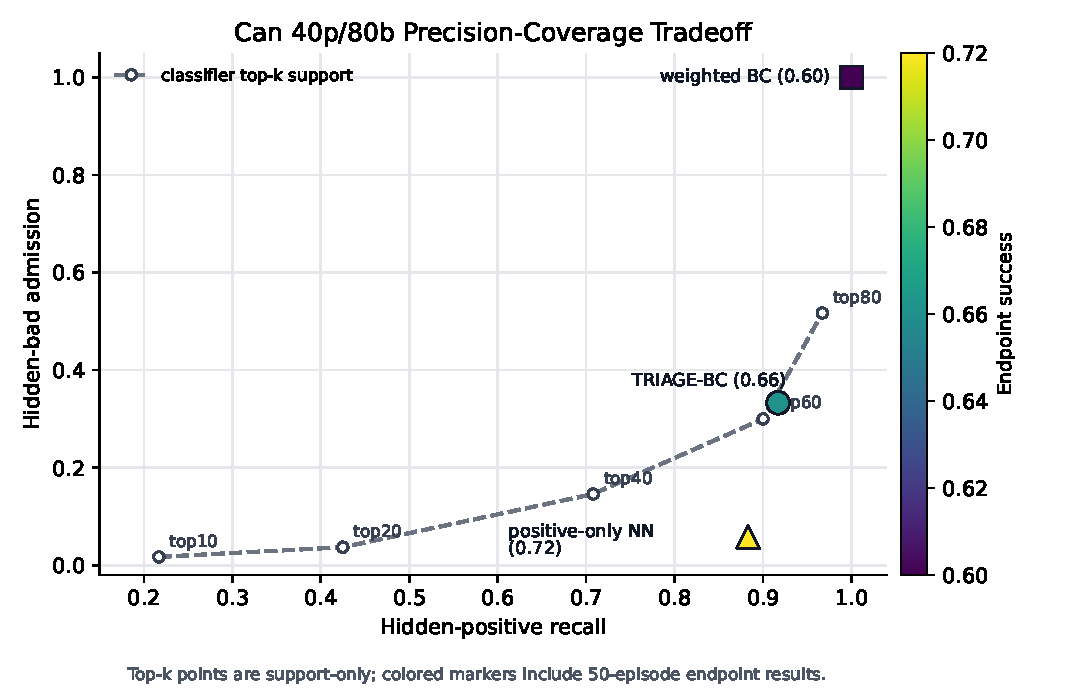
\includegraphics[width=\linewidth]{../results/final_paper/figures/can40_precision_coverage.pdf}
  \caption{Can 40p/80b precision/coverage analysis. Bad labels improve score calibration, but the current converter can sit off the best precision/coverage frontier relative to positive-only retrieval.}
  \label{fig:precision}
\end{figure}

\subsection{Score Shape and Abstention}

Score-shape diagnostics explain why no single converter works everywhere. Can 40p/80b has moderate positive/bad overlap, motivating adaptive mass-capped hard support. Lift MG has stronger score separation, but policy performance still favors weighted coverage. Can MG has a high-score plateau containing both positives and bad demos, which motivates router abstention.

\begin{figure}[t]
  \centering
  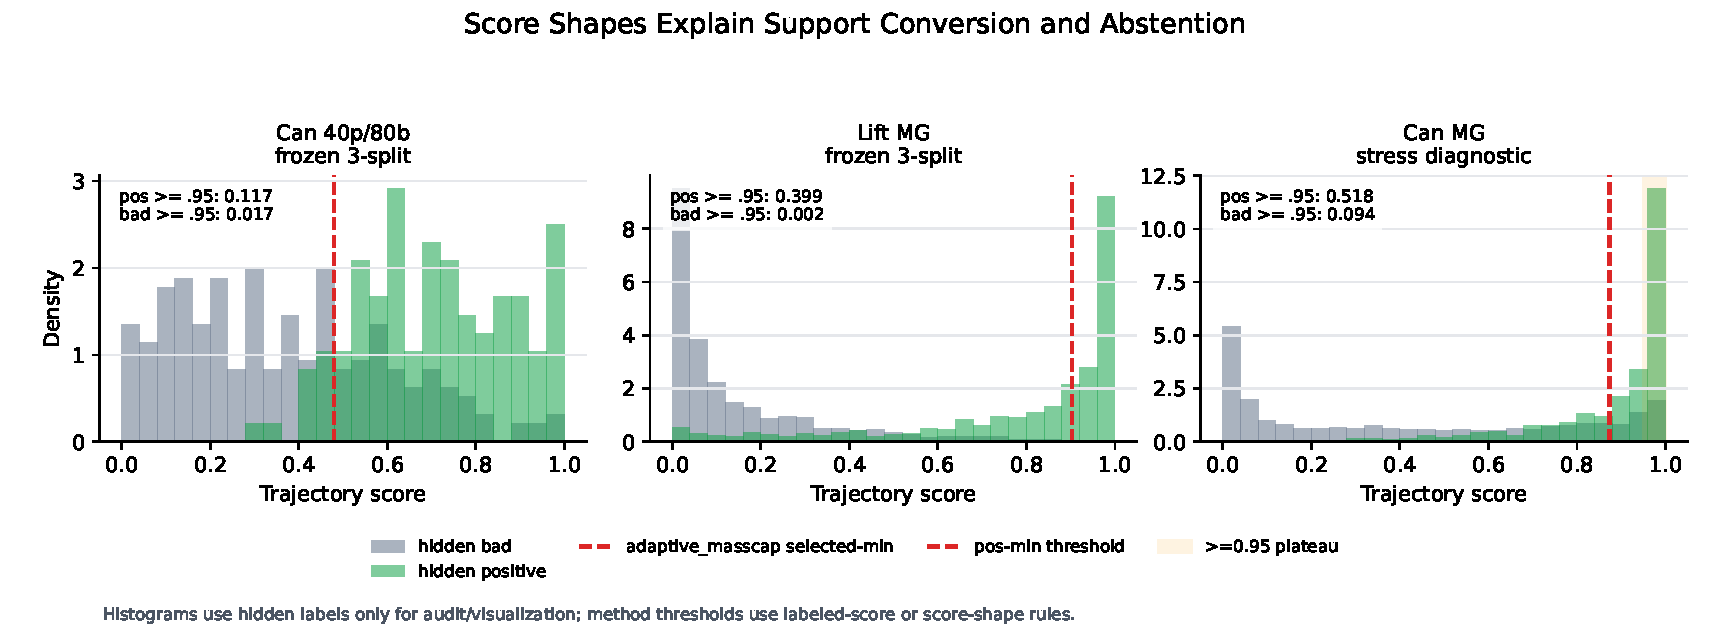
\includegraphics[width=\linewidth]{../results/final_paper/figures/score_shape_diagnostics.pdf}
  \caption{Score-shape diagnostics. High-purity support is not sufficient evidence of policy quality when coverage dominates or when high-score plateaus remain ambiguous.}
  \label{fig:score-shapes}
\end{figure}

The Can MG branch-proxy diagnostic shows that simple positive and negative likelihood proxies are not enough. On original Can MG, the rollout-best fixed-20k method is weighted BC, but the tested likelihood proxies choose all-positive support. On shuffled Can MG, proxy selection cannot detect that both hard and soft branches are weak. This supports abstention rather than overconfident branch choice.

\subsection{Precision/Coverage View}

The results can be summarized by two audit-only quantities: hidden-positive recall and hidden-bad admission. Hard selection helps when it removes action-conflicting bad support faster than it loses useful coverage, and fails when discarded trajectories contain coverage that the sequence policy needs. This explains the reversals: Can 40p/80b contains action-conflicting contamination, so \method{} can beat weighted BC even though positive-only NN finds a cleaner frontier; Lift MG favors broader weighted coverage despite purer hard support. The target for future work is therefore a hidden-label-free policy-quality proxy that predicts when added coverage is worth added contamination.

\section{A Simple Precision/Coverage Analysis}

This section gives a lightweight model for the empirical precision/coverage tradeoff. It is not a formal guarantee for nonlinear sequence BC; it is an organizing decomposition that explains why neither the purest support nor the broadest weighted support is uniformly optimal.

Assume the unlabeled log is a mixture of hidden useful and harmful trajectories,
\begin{equation}
  \Dunl \sim \pi_g P_g + (1-\pi_g)P_b,
\end{equation}
where $P_g$ denotes desirable hidden support and $P_b$ denotes harmful or action-conflicting support. A threshold or support rule induces a selected set $S_t \subseteq \Dunl$ with hidden-good recall $r_t$ and hidden-bad admission $f_t$. If $N_g$ and $N_b$ are the hidden-good and hidden-bad counts in $\Dunl$, then $r_tN_g$ useful trajectories reduce estimation and coverage error, while $f_tN_b$ harmful trajectories create an imitation-contamination penalty.

A schematic excess-risk decomposition for behavior cloning on $\Dpos\cup S_t$ is
\begin{equation}
  \mathcal{R}(\hat{\pi}_t) - \mathcal{R}(\pi_g)
  \;\lesssim\;
  \underbrace{\frac{A}{\sqrt{n_+ + r_tN_g}}}_{\text{coverage / estimation}}
  +
  \underbrace{
  C\frac{f_tN_b}{n_+ + |S_t|}
  }_{\text{bad-action contamination}},
  \label{eq:hard-risk-view}
\end{equation}
for task-dependent constants $A$ and $C$. The first term favors larger selected support when useful state-action coverage is scarce. The second term favors more selective support when admitted bad trajectories contain actions that conflict with the desired behavior. The optimal support threshold is therefore not necessarily the purest threshold: when the coverage term dominates, admitting additional imperfect trajectories can still improve policy learning.

\paragraph{Marginal support criterion.}
The decomposition also gives a simple one-step test for whether adding another unlabeled trajectory should help. Let $m_t=|S_t|$, $g_t=r_tN_g$, and $b_t=f_tN_b$. Suppose a candidate trajectory is useful with probability $q$ under the score model and harmful with probability $1-q$. Under Eq.~\ref{eq:hard-risk-view}, adding it decreases the bound whenever
\begin{equation}
  A\left(
  \frac{1}{\sqrt{n_+ + g_t}} -
  \frac{1}{\sqrt{n_+ + g_t + q}}
  \right)
  >
  C\left(
  \frac{b_t + 1 - q}{n_+ + m_t + 1} -
  \frac{b_t}{n_+ + m_t}
  \right).
  \label{eq:marginal-support}
\end{equation}
The left side is the expected coverage gain; the right side is the expected increase in bad-action mass after normalizing by the enlarged training set. This inequality makes the empirical reversals concrete. A pure but tiny support can be suboptimal when the left side remains large for moderately risky coverage trajectories. Conversely, hard filtering wins when extra trajectories mostly increase the right side because they are action-conflicting failures.

For a weighted sampler with trajectory weights $w(\tau)$, the analogous view replaces selected count with effective sample size and bad count with bad weight mass:
\begin{equation}
  \mathcal{R}(\hat{\pi}_w) - \mathcal{R}(\pi_g)
  \;\lesssim\;
  \underbrace{\frac{A}{\sqrt{n_+ + \operatorname{ESS}(w)}}}_{\text{weighted coverage}}
  +
  \underbrace{
  C\frac{\sum_{\tau\in P_b}w(\tau)}
          {n_+ + \sum_{\tau\in\Dunl}w(\tau)}
  }_{\text{weighted bad-action mass}},
  \label{eq:weighted-risk-view}
\end{equation}
where $\operatorname{ESS}(w)=(\sum_\tau w(\tau))^2/\sum_\tau w(\tau)^2$. Soft weighting can win when broad coverage is essential and bad-action mass is low or weakly conflicting. Hard support can win when bad-action mass is high and score rankings can remove it without losing too much useful coverage.

\method{} v0.1 can be read as a hidden-label-free approximation to these two terms. The positive-mass estimate $\hat{m}$ limits selected support when the score shape suggests that additional trajectories are more likely to add contamination than coverage. The positive-minimum branch broadens support when labeled positives occupy a high-score region with many unlabeled neighbors. The abstention branch handles score shapes where the method cannot reliably estimate the balance between the two terms. This analysis also explains why positive-only retrieval is a critical baseline: it can lie on a better precision/coverage frontier even without negative labels.

\section{Discussion and Limitations}

The main empirical lesson is that tri-signal labels are useful, but their value is mediated by support conversion. A classifier score is not the policy. A high-purity selected set is not always enough. A broad weighted set is not always safe. Different tasks occupy different parts of the precision/coverage landscape.

The strongest positive result is not universal dominance. It is that hard selected support can improve over weighted BC and all-demo cloning on Can contamination, and that a frozen v0.2 portfolio can choose hard union on fresh Can while switching to weighted coverage on fresh Lift. Controlled PointNav and generated Can diagnostics explain why scarce bad labels can be mechanistically valuable; the limitation is that positive-only NN is often stronger on Can and weighted BC remains the right branch on Lift-like broad-coverage rows.

TRIAGE-BC is a score-calibrated imitation method using a strong BC-RNN-GMM backbone, not a validated inverse-Q robotics method. Positive-only NN is the strongest non-oracle row on the original Can 40p/80b matrix and completed Can 20p/80b diagnostic; Weighted BC is strongest on the original Lift MG matrix and selected by v0.2 on fresh Lift. Can MG remains a stress diagnostic where abstention is more honest than claiming success on ambiguous high-score plateaus.

The evaluation uses 50 endpoint rollouts per split. This is stronger than earlier 10-episode screens, but repeated rollouts from the same validation-positive start pool are not fully independent. Claims should report split-level and endpoint-count context.

\section{Conclusion}

\method{} reframes offline imitation from scarce successes, scarce failures, and mixed logs as a score-to-support conversion problem. The results show that tri-signal scores can recover useful hidden support, that hard support can beat soft weighting in some contaminated settings, and that a frozen portfolio router can improve a fresh Can+Lift gate by selecting different support conversions in different regimes. They also show that strong no-bad-label retrieval and broad weighted coverage are essential baselines. The central claim is therefore precise: support calibration is the bottleneck, and reliable hidden-label-free conversion from scores to policy-training data is the next algorithmic step.

\appendix

\section{Diagnostic Endpoint and Support Evidence}

Figure~\ref{fig:diagnostic-matrix} shows the broader endpoint matrix that includes diagnostic Can 20p/80b and Can 80p/80b rows. These rows are not promoted to main claims because they are not complete three-split endpoint tables. They are included to document the precision/coverage caveat and the strength of positive-only retrieval.

\begin{figure}[t]
  \centering
  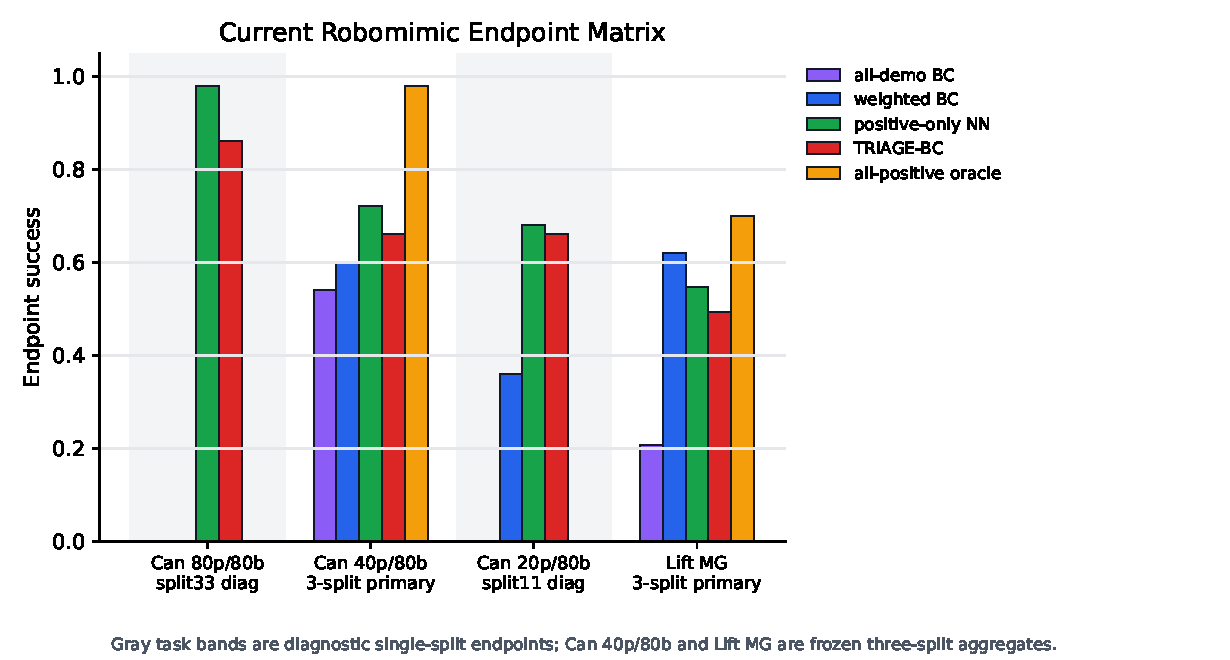
\includegraphics[width=\linewidth]{../results/final_paper/figures/robotics_current_endpoint_matrix.pdf}
  \caption{Broader Robomimic endpoint matrix. Can 20p/80b and Can 80p/80b are diagnostic rows; the primary main-paper matrix is restricted to completed three-split Can 40p/80b and Lift MG aggregates.}
  \label{fig:diagnostic-matrix}
\end{figure}

Figure~\ref{fig:paired-deltas} visualizes the paired initial-state deltas behind the primary bootstrap audit. It makes the repeated-start structure explicit: endpoint gaps are visible at the validation-start level, but the bootstrap intervals for the primary Can and Lift method comparisons mostly cross zero.

\begin{figure}[t]
  \centering
  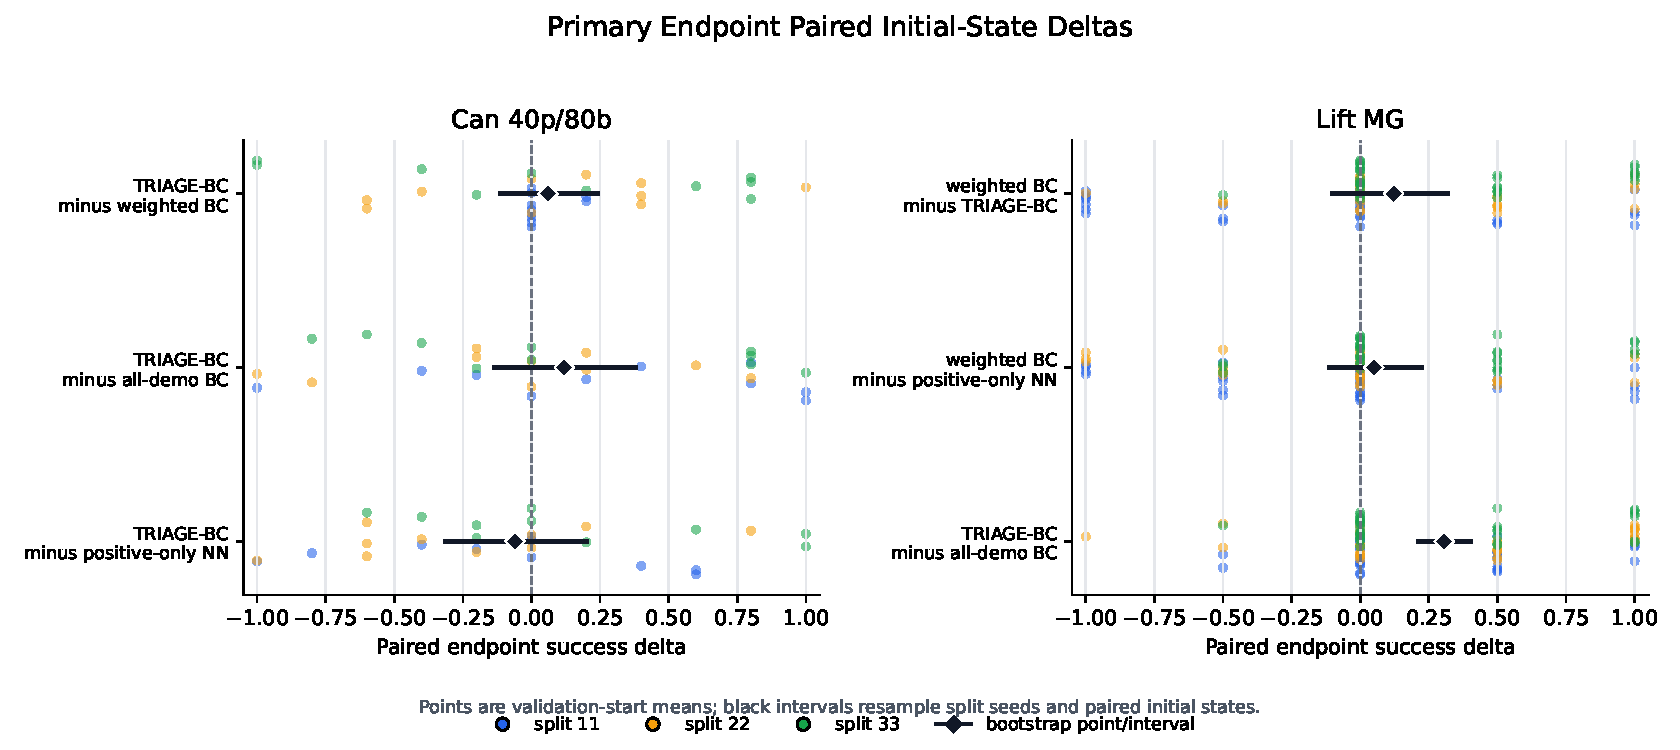
\includegraphics[width=\linewidth]{../results/final_paper/figures/primary_endpoint_paired_deltas.pdf}
  \caption{Paired endpoint success deltas by held-out validation initial state. Points average repeated rollouts from the same initial state; black intervals resample split seeds and paired initial states.}
  \label{fig:paired-deltas}
\end{figure}

Figure~\ref{fig:prefix-positive-can} shows the strongest generated Can diagnostic. It mirrors the PointNav prefix-positive setup in Robomimic: trusted positives are only early successful-demo prefixes, while full successful and failed demonstrations are hidden in the unlabeled pool.

\begin{figure}[t]
  \centering
  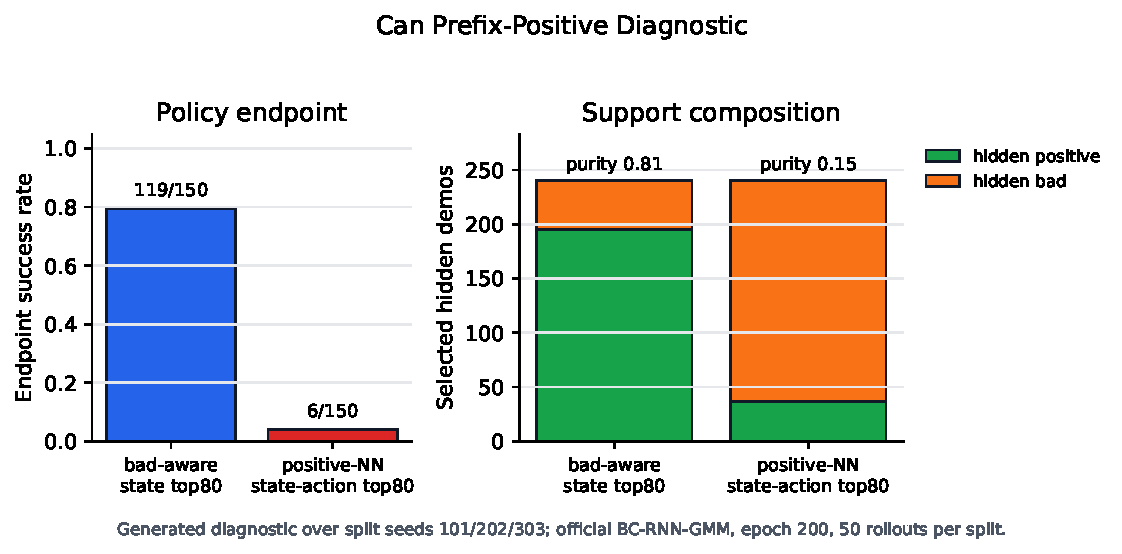
\includegraphics[width=\linewidth]{../results/final_paper/figures/can_prefix_positive_diagnostic.pdf}
  \caption{Generated Can prefix-positive diagnostic over split seeds 101/202/303. Explicit failures let the bad-aware selector recover far cleaner full-trajectory support and transfer to the BC-RNN-GMM endpoint, but this remains a generated diagnostic rather than a primary benchmark row.}
  \label{fig:prefix-positive-can}
\end{figure}

Table~\ref{tab:bad-label-controls} consolidates the bad-label control evidence. It is an appendix guardrail: explicit failures are useful calibration signal, but the current converter is not a universal improvement over strong positive-only retrieval. The Can 40p/80b row is the clearest caveat: \method{} recovers 110 versus 106 hidden positives but admits 80 versus 14 hidden bad demos.

\begin{table}[t]
  \centering
  \scriptsize
  \setlength{\tabcolsep}{3pt}
  \resizebox{\linewidth}{!}{%
  \begin{tabular}{@{}llll@{}}
    \toprule
    Setting & Bad-aware endpoint & No-bad/control endpoint & Support audit \\
    \midrule
    PointNav $n_+=5$, $n_-\in\{1,2,5\}$ & gap support 0.973/0.997 min/mean & BC-all 0.292; local weighted 0.131 & purity 1.000, 0 hidden-bad demos \\
    Can 40p/80b & \method{} 99/150 & positive-only NN 108/150 & 110 pos/80 bad vs 106 pos/14 bad \\
    Can 20p/80b & \method{} 46/100 & positive-only NN 54/100 & 54/69 vs 49/11 hidden pos/bad \\
    Can 80p/80b & \method{} 43/50 & positive-only NN 49/50 & 137/28 vs 220/20 hidden pos/bad \\
    Lift MG & \method{} 74/150 & positive-only NN 82/150 & 421/20 vs 342/138 hidden pos/bad \\
    \bottomrule
  \end{tabular}}
  \caption{Bad-label versus positive-only control summary. The table separates calibration/support evidence from endpoint superiority claims.}
  \label{tab:bad-label-controls}
\end{table}

Table~\ref{tab:hard-negative-can} adds a targeted generated hard-negative Can diagnostic. The split construction intentionally makes some bad demos close in state space to labeled positives while disagreeing in action, so state-action positive-only retrieval is a strong but vulnerable baseline. Under the same BC-RNN-GMM endpoint protocol, a bad-aware rank-fusion hybrid keeps substantially cleaner support and improves endpoint success over state-action positive-NN top40. This is evidence that explicit failures can matter when the unlabeled bad demos are action-conflicting near-neighbors, but it remains a generated diagnostic rather than a primary benchmark row.

\begin{table}[t]
  \centering
  \scriptsize
  \setlength{\tabcolsep}{4pt}
  \begin{tabular}{@{}lrrrr@{}}
    \toprule
    Support rule & hidden pos & hidden bad & endpoint & avg len \\
    \midrule
    Bad-aware hybrid top40 & 113 & 7 & 104/150 & 198.9 \\
    State-action positive-NN top40 & 70 & 50 & 91/150 & 223.3 \\
    \bottomrule
  \end{tabular}
  \caption{Generated hard-negative Can endpoint diagnostic over split seeds 101/202/303. Per-split endpoint counts are 33/50 versus 30/50, 35/50 versus 27/50, and 36/50 versus 34/50 for the bad-aware hybrid versus state-action positive-NN baseline.}
  \label{tab:hard-negative-can}
\end{table}

Table~\ref{tab:coverage-shift-can} gives a second generated Can diagnostic. Here labeled positives come from a narrow initial-object-pose cluster, while hidden positives cover the remaining successful clusters and hidden bad demos are spread across initial conditions. This setting tests whether bad-aware scoring can recover useful support outside the trusted-positive coverage region without admitting failures. The bad-aware-heavy hybrid improves endpoint success and selects cleaner support than state-action positive-NN top40, but this row is still a targeted generated diagnostic rather than a primary benchmark result.

\begin{table}[t]
  \centering
  \scriptsize
  \setlength{\tabcolsep}{4pt}
  \begin{tabular}{@{}lrrrr@{}}
    \toprule
    Support rule & hidden pos & hidden bad & endpoint & avg len \\
    \midrule
    Bad-aware-heavy hybrid top40 & 118 & 2 & 120/150 & 182.7 \\
    State-action positive-NN top40 & 105 & 15 & 103/150 & 207.5 \\
    \bottomrule
  \end{tabular}
  \caption{Generated coverage-shift Can endpoint diagnostic over split seeds 101/202/303. Per-split endpoint counts are 39/50 versus 35/50, 41/50 versus 29/50, and 40/50 versus 39/50 for the bad-aware-heavy hybrid versus state-action positive-NN baseline.}
  \label{tab:coverage-shift-can}
\end{table}

The appendix diagnostics are:
\begin{itemize}[leftmargin=*]
  \item \textbf{Controlled PointNav label efficiency.} With only 2 positive route-prefix demos and 2 bad shortcut demos, gap-demo BC reaches 1.000 success at 50/75/90/95\% bad unlabeled data. With 5 positives and 1/2/5 labeled bad shortcuts, the selected support has 1.000 demo purity, 1.000 transition purity, and 0 hidden-bad demos in every row. The 1 labeled bad shortcut and 5 labeled bad shortcut settings both reach 1.000 gap-demo success at every tested contamination level; the 2-bad setting remains near-perfect but dips to 0.973 and 0.993 at 90\% and 95\% bad data. This supports label efficiency for the controlled mechanism, not a claim that bad labels are necessary on Can.
  \item \textbf{Can 20p/80b.} The three-split support audit plus two completed endpoint splits show positive-only NN at 54/100 endpoint successes, \method{} at 46/100, and weighted BC at 18/50 on split 11. \method{} recovers more hidden positives than positive-only NN, 54/60 versus 49/60, but admits many more hidden bad demos, 69/240 versus 11/240.
  \item \textbf{Can 80p/80b.} The three-split support audit plus split-33 endpoint show positive-only NN at 49/50 and \method{} at 43/50. Even when \method{} selects purer split-33 support, positive-only retrieval keeps better coverage and wins the endpoint.
  \item \textbf{Can MG.} The branch-proxy diagnostic shows that original Can MG is rollout-best with weighted BC at 0.333, while simple positive and negative likelihood proxies choose all-positive support at 0.200. These proxies do not replace abstention because they miss coverage-sensitive rollout quality.
  \item \textbf{Hard-negative Can.} A generated three-split action-conflict diagnostic reverses the positive-only caveat: the bad-aware hybrid reaches 104/150 endpoint successes and selects 113 hidden positives with only 7 hidden bad demos, while state-action positive-NN top40 reaches 91/150 and selects 70 hidden positives with 50 hidden bad demos. This supports explicit bad-label utility under near-neighbor action conflict, not a claim of primary benchmark dominance.
  \item \textbf{Coverage-shift Can.} A generated three-split scarce-positive coverage-shift diagnostic gives the bad-aware-heavy hybrid 120/150 endpoint successes and selects 118 hidden positives with only 2 hidden bad demos, while state-action positive-NN top40 reaches 103/150 and selects 105 hidden positives with 15 hidden bad demos. This supports explicit bad-label utility when trusted positives under-cover initial conditions, not a primary benchmark dominance claim.
  \item \textbf{Prefix-positive Can.} In a generated three-split diagnostic where trusted positives are early successful-demo prefixes and full demos are unlabeled, prefix bad-aware state top80 reaches 119/150 and selects 195 hidden positives with 45 hidden bad, versus prefix state-action positive-NN top80 at 6/150 with 37 hidden positives and 203 hidden bad. This mirrors PointNav and is diagnostic only.
  \item \textbf{Action-risk v0.2 no-go.} A support-side action-risk family can dominate positive-only support labels, but endpoint checks show that support purity alone is still not a policy-quality proxy. On Can 40p/80b split 11, positive-NN/risk fusion selects 39 hidden positives and 1 hidden bad demo but reaches 0.820 success, below positive-only NN at 0.840. On split 22, it selects 40 hidden positives and 0 hidden bad demos but reaches 0.640, below positive-only NN at 0.760. This rejects the current action-risk candidate as \method{} v0.2 and motivates abstention or stronger policy-quality prediction.
  \item \textbf{Lift MG classifier top160.} The fixed classifier-score top160 ablation reaches 68/150 pooled successes, below \method{} at 74/150, positive-only NN at 82/150, and weighted BC at 93/150. A broader high-purity classifier top-k rule does not rescue Lift; policy quality needs more than support purity.
\end{itemize}

The diagnostic rows are consistent with the main claim. Bad labels can improve score calibration and hard support can beat soft weighting on the completed Can 40p/80b matrix, but the current converter is not on the best Can precision/coverage frontier. Positive-only retrieval is cleaner on Can 20p/80b and stronger on the Can 80p/80b endpoint diagnostic. The generated hard-negative, coverage-shift, and prefix-positive diagnostics show settings where explicit failures help beyond positive-only retrieval, while Can MG shows that simple branch-quality proxies are inadequate and Lift MG shows that high-purity support can still under-cover the policy learner.

\section{Reproducibility and Artifact Map}

The paper-facing method contract is fixed in \path{../METHOD_FREEZE.md}, with
run and evaluation settings in \path{../configs/final_method.yaml} and
\path{../configs/final_eval.yaml}. Cheap regeneration commands and the full
artifact-to-script map are documented in \path{../paper/REPRODUCE_PAPER.md}.
Primary Robomimic rows use split seeds 11, 22, and 33, policy seed 0, fixed
epoch-200 checkpoints, and 50 held-out validation-positive endpoint rollouts per
split. Key report paths are:
\begingroup
\footnotesize
\sloppy
\raggedright
  \begin{itemize}[leftmargin=*]
  \item Mechanism and primary matrix:
        \path{../results/final_paper/tables/pointnav_controlled_mechanism_REPORT.md};
        \path{../results/final_paper/tables/robotics_primary_endpoint_matrix_REPORT.md}.
  \item Primary uncertainty:
        \path{../results/final_paper/tables/primary_endpoint_paired_bootstrap_REPORT.md};
        \path{../results/final_paper/tables/primary_endpoint_paired_deltas_REPORT.md}.
  \item Fresh v0.2 gate:
        \path{../results/final_paper_v02/tables/v02_fresh_gate_REPORT.md};
        \path{../results/final_paper_v02/tables/v02_fresh_gate_uncertainty_REPORT.md};
        \path{../results/final_paper_v02/tables/v02_fresh_router_support_REPORT.md}.
  \item Controls and generated diagnostics:
        \path{../results/final_paper/tables/bad_label_control_summary_REPORT.md};
        \path{../results/final_paper/ablations/hard_negative_can_endpoint_200ep/REPORT.md};
        \path{../results/final_paper/ablations/can_coverage_shift_endpoint_200ep/REPORT.md};
        \path{../results/final_paper/tables/can_prefix_positive_diagnostic_REPORT.md}.
\end{itemize}
\endgroup

\bibliographystyle{plain}
\bibliography{references}

\end{document}
